% figs/lattice_potential.tex  – 1-D sinusoidal lattice potential
\begin{tikzpicture}[x=0.8cm, y=0.55cm, >=stealth, font=\small]
  % axes
  \draw[->] (-0.3,0) -- (6.4,0) node[below] {$x$};
  \draw[->] (0,-1.1) -- (0,1.3) node[left] {$V(x)$};

  % potential V(x)=sin x
  \draw[thick, blue!70, samples=200, smooth, domain=0:6.2]
        plot (\x,{sin(\x r)});

  % minima markers
  \foreach \k in {1,3,5}{
    \fill [red!70] (\k*pi/2,0) circle [radius=1.2pt];
  }

  % label
  \node[above right] at (4.2,-0.7) {$V_0\sin\!\bigl(\tfrac{2\pi}{a}x\bigr)$};
\end{tikzpicture}
